%!TEX program =pdflatex
\documentclass{beamer}

%%define new comand
\def\argmin{\mathop{\rm arg~min}\limits}
\newcommand{\suit}[1]{\left(#1\right)}
\newcommand{\abs}[1]{\left\vert#1\right\vert}
\newcommand{\set}[1]{\left\{#1\right\}}
\newcommand{\bra}[1]{\left[ #1 \right]}
\usetheme{CambridgeUS}
\title{Distributed Inference for Extreme Value Index}
\date{}
\author{Liujun Chen}

\begin{document}
\begin{frame}
\titlepage
\begin{center}
    \vspace{-17ex}


 Fudan University

    \bigskip

    joint work with Deyuan Li and Chen Zhou

    \bigskip
    On Extreme Value Analysis 2021
\end{center}
\end{frame}

\begin{frame}
    \frametitle{ Distributed Inference}

    


\begin{itemize}


    \item Data privacy issue.
    \medskip
    \begin{itemize}
        \item Bank may not share their operational loss.
        \medskip
        \item Insurance firms cannot share insurance claims.
    \end{itemize}
    
    \pause
    \bigskip
    \bigskip
    \item Computational issue.
     \medskip
    \begin{itemize}
        \item Size of the dataset is beyond a computer's memory.
    \end{itemize}
   
\end{itemize}
    

\end{frame}


\begin{frame}
    \frametitle{Distributed Inference}
    \begin{itemize}
        \item Divide and Conquer algorithm:
    \begin{itemize}
        \medskip
        \item estimates on each machine 
        \medskip
        \item transmits the results to the center machine
        \medskip
        \item takes "average" in the central machine
    \end{itemize}
        
        \bigskip
        \pause
        \item {\color{red} Oracle Property}
    
        Whether the aggregated estimator achieves the same statistical efficiency as the {\color{blue} Oracle estimator} (the imaginary estimator using all observations).
    \end{itemize} 
\end{frame}


% \begin{frame}
%     \frametitle{Divide and Conquer Algorithm}
% {\bf Estimating the extreme value index}

% \bigskip
%     \begin{itemize}
%         \item Assume $N$ i.i.d. observations are stored in $m$ machines with $n$ observations in each machine.
%         \medskip
%         \item Apply the Hill estimator to each machine. 
%         \medskip
%         \item Transmit the results to a central machine.
%         \medskip
%         \item Take the average of the Hill estimates from all machines.
%         \medskip
%         \item We call the final estimator "distributed Hill estimator".
%     \end{itemize}
    

% \end{frame}


\begin{frame}
    \frametitle{Model Setting}
\begin{itemize}
    \item Consider a distribution function $F\in D(G_{\gamma})$ with $\gamma>0$ (heavy tailed distribution).
    \bigskip
    \item This is equivalent to that $U:=\set{1/(1-F)}^{\leftarrow}$ is a regular varying function:
    $$
        \lim_{t\to\infty} \frac{U(tx)}{U(t)} = x^{\gamma}.
    $$
    \bigskip
    \item A key question in extreme value analysis is to estimate the extreme value index.
\end{itemize}
    

\end{frame}


\begin{frame}
    \frametitle{Model Setting}
\begin{itemize}
    \item Assume that the i.i.d. observations $X_1,\dots,X_N$ are stored in $m$ machines with $n$ observations in each machine, i.e. $N = nm$.
    \bigskip
    \item Assume that $m = m(N)\to\infty, n= n(N)\to \infty$ as $N\to\infty$.
    \bigskip
    \item Practically, we cannot apply statistical procedures to the oracle
    sample, i.e, the hypothetically combined dataset $\set{X_1,\dots,X_N}$.
\end{itemize}
    

\end{frame}


\begin{frame}
    \frametitle{Oracle Hill estimator}
    If we can use the oracle sample, the (oracle) Hill estimator is defined as
    $$
        \hat{\gamma}_H: = \frac{1}{l}\sum_{i=1}^{l} \log M^{(i)}-\log M^{(l+1)}
    $$
    where $l = l(N)\to \infty, l/N \to 0$ as $N\to \infty$.
   
    Here, $M^{(1)} \ge \cdots \ge  M^{(N)}$ are the order statistics of the oracle sample.

\end{frame}

\begin{frame}
    \frametitle{Distributed Hill estimator}
Following a divide and conquer algorithm:

\medskip
\begin{itemize}
    \item Apply the Hill estimator at each machine:
    $$
        \hat{\gamma}_{j,H} = \frac{1}{k}\sum_{i=1}^{k} \log M_{j}^{(i)} -\log M_j^{(k+1)}.
    $$
    Here, $M^{(1)}_j \ge \cdots \ge M_j^{(n)}$ are the order statistics of the observations in machine $j$.
    \medskip
    \item Take the average of the Hill estimates from all machines
    $$
    \hat{\gamma}_{DH}:=\frac{1}{m}\sum_{j=1}^m \hat{\gamma}_{j,H}.
    $$
\end{itemize}
    
\end{frame}


\begin{frame}

    \frametitle{Main Conditions}

\begin{itemize}
    \item[(A)] $m = m(N)\to\infty, n= n(N)\to\infty$ and $n/\log m\to\infty$ as $N\to\infty$. 
    \bigskip
    \item[(B)] (Second Order Condition.)  There exist an eventually positive or negative function $A$ with $\lim_{t\to\infty} A(t)=0$ and a real number $\rho\le 0$ such that
    $$
    \lim_{t\to\infty} \frac{\frac{U(tx)}{U(t)}-x^{\gamma}}{A(t)} = x^{\gamma}\frac{x^{\rho}-1}{\rho},
    $$
    for all $x\ge 0$.
\end{itemize}
    

\end{frame}

\begin{frame}
    \frametitle{Asymptotics: when $k$ is fixed}
{\bf{Theorem }}
    Suppose that $F\in D(G_{\gamma})$ with $\gamma>0$ and Conditions $A$ and $B$ hold. Assume $k\ge 1$ is a fixed integer. If $\sqrt{km}A(n/k) = O(1)$ as $N\to\infty$,
    $$
\sqrt{km}\set{\hat{\gamma}_{DH}-\gamma-A(n/k)g(k,n,\rho)}\stackrel{d}{\to} N(0,\gamma^2),
    $$
where
$$
g(k,n,\rho) = \frac{1}{\rho}\suit{\frac{n}{k}}^{-\rho} \frac{\Gamma(n+1)\Gamma(k-\rho+1)}{\Gamma(n-\rho+1)\Gamma(k+1)}.
$$
\end{frame}


\begin{frame}
\frametitle{Oracle Property: when $k$ is fixed}
\begin{itemize}
    \item Assume that $\sqrt{km}A\suit{\frac{N}{km}} =\sqrt{km}A\suit{\frac{n}{k}}\to\lambda \in \mathbb{R}$, the Oracle Hill estimator possesses the asymptotic normality 
    $$
    \sqrt{km}\suit{\hat{\gamma}_H-\gamma}\stackrel{d}{\to} N(\lambda/(1-\rho), \gamma^2).
    $$
    \pause
    \medskip
    \item Under the same condition, we have that
    $$
        \sqrt{km}\suit{\hat{\gamma}_{DH}-\gamma}\stackrel{d}{\to} N\suit{\lambda\frac{k^{\rho}}{1-\rho}\frac{\Gamma(k-\rho+1)}{\Gamma(k+1)},\gamma^2}.
    $$
    \medskip
    \pause
    \item The oracle property holds only when $\rho= 0$ or $\lambda = 0$.
\end{itemize}
    


\end{frame}


\begin{frame}
    \frametitle{Asymtotics: when $k$ is an intermediate sequence}
{\bf Theorem } Suppose $F\in D(G_{\gamma})$ with $\gamma>0$ and Conditions $A$ and $B$ hold. Assume $k = k(N)\to\infty, k/n \to 0$ as $N\to\infty$. If $\sqrt{km}A\suit{n/k} =O(1)$, then
$$
\sqrt{km}\set{\hat{\gamma}_{DH}-\gamma-A(n/k) g(k,n,\rho)}\stackrel{d}{\to} N(0,\gamma^2).
$$
    

\end{frame}

\begin{frame}
    \frametitle{Oracle property: when $k$ is an intermediate sequence }
    \begin{itemize}
        \item Assume that $\sqrt{km}A\suit{\frac{N}{km}} =\sqrt{km}A\suit{\frac{n}{k}}\to\lambda \in \mathbb{R}$, the Oracle Hill estimator possesses the asymptotic normality 
        $$
        \sqrt{km}\suit{\hat{\gamma}_H-\gamma}\stackrel{d}{\to} N(\lambda/(1-\rho), \gamma^2).
        $$
        \pause
        \medskip
        \item Under the same condition, $g(k,n,\rho)\to 1$, we have that
        $$
            \sqrt{km}\suit{\hat{\gamma}_{DH}-\gamma}\stackrel{d}{\to} N\suit{\frac{\lambda}{1-\rho},\gamma^2}.
        $$
        \medskip
        \pause
        \item The oracle property always holds in this case.
    \end{itemize}
\end{frame}




\begin{frame}
    \frametitle{Simulation: squared bias for different level of $k$}

\begin{center}
    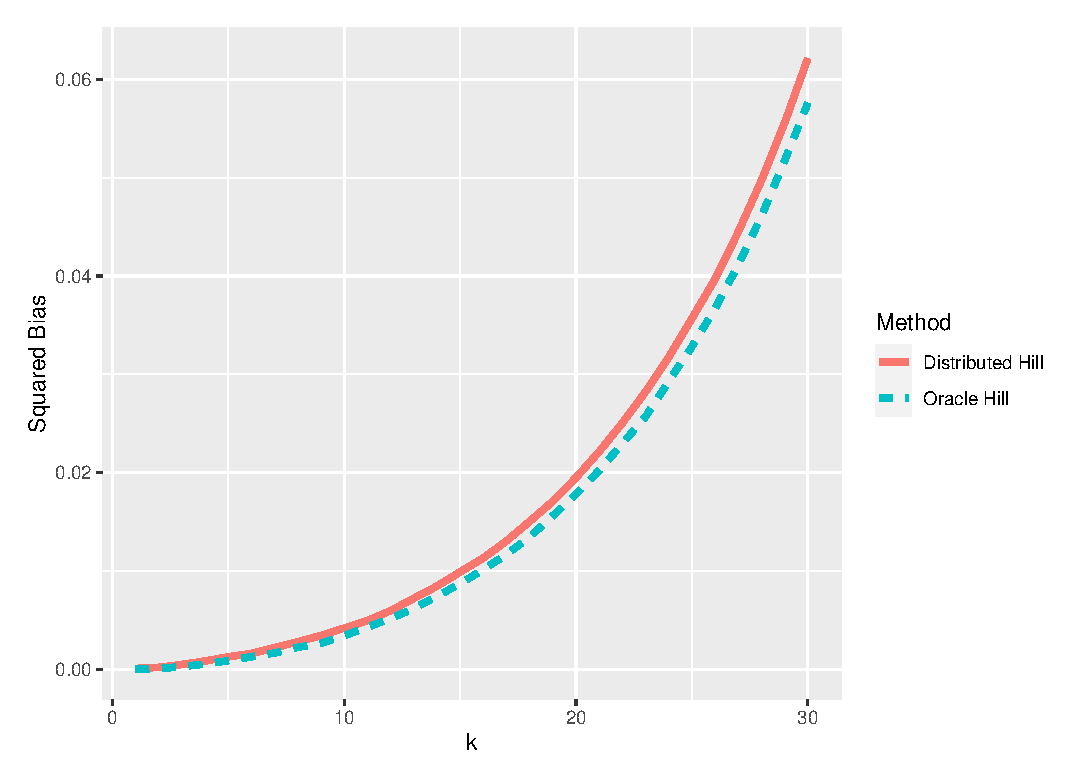
\includegraphics[width = 0.5\textwidth]{Simulation/Frechet_20_50_choice_d_bias.eps} 
\end{center}

\begin{itemize}
    \item Unit Fr\'echet distribution ($\rho=-1$), $N=1000, m=20,n=50$
    \item Oracle Hill estimator uses $km =20k$ exceedance ratios
\end{itemize}
\end{frame}



\begin{frame}
    \frametitle{Simulation: variance for different level of $k$}
    \begin{center}
         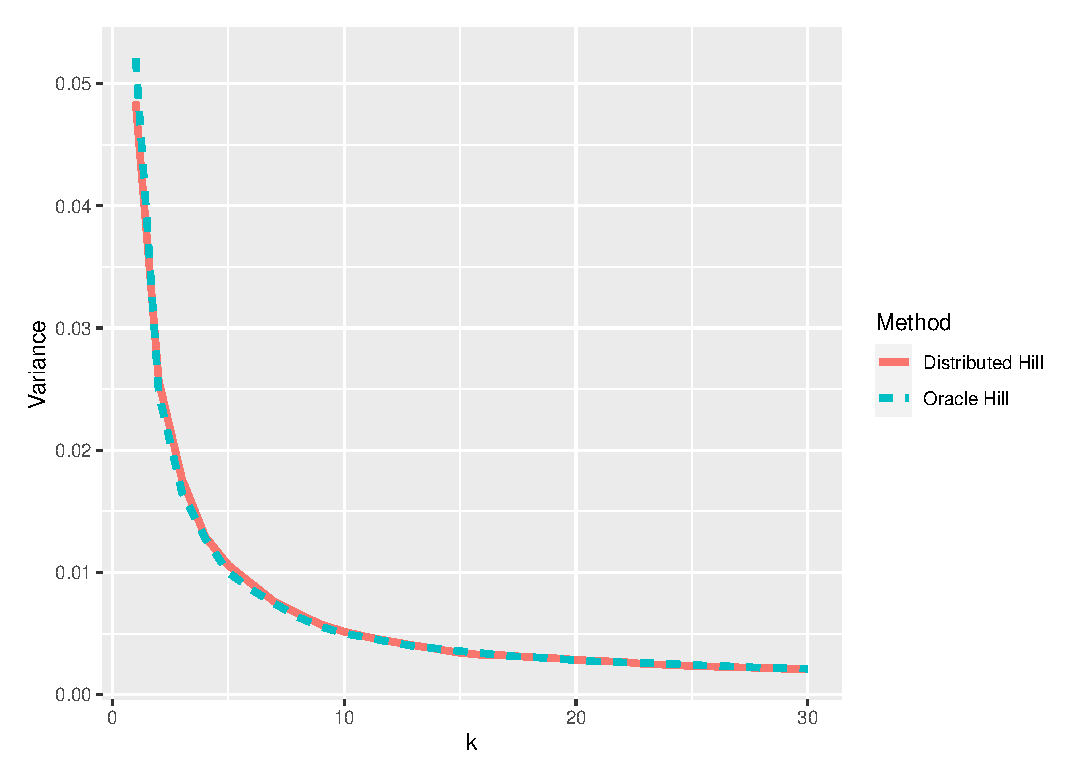
\includegraphics[width = 0.5\textwidth]{Simulation/Frechet_20_50_choice_d_variance.eps} 
    \end{center}
    \begin{itemize}
        \item Unit Fr\'echet distribution ($\rho=-1$), $N=1000, m=20,n=50$
        \item Oracle Hill estimator uses $km =20k$ exceedance ratios
    \end{itemize}
\end{frame}



\begin{frame}
    \frametitle{Simulation: MSE for different level of $k$}
    \begin{center}
         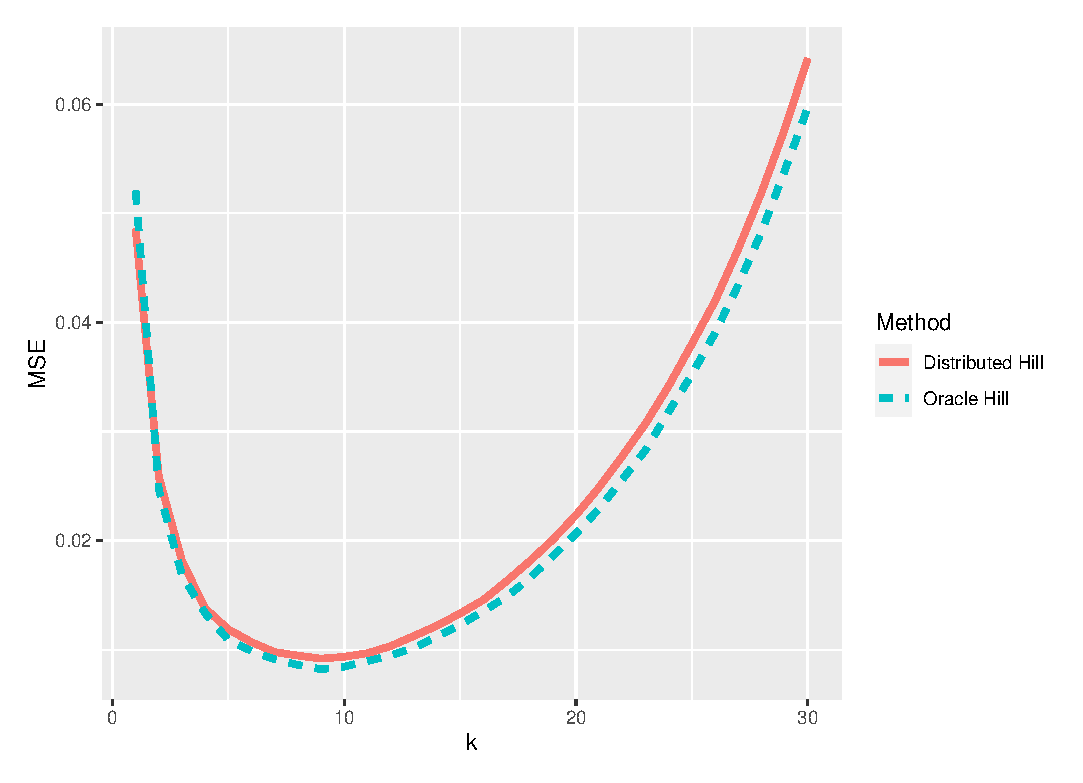
\includegraphics[width = 0.5\textwidth]{Simulation/Frechet_20_50_choice_d_mse.eps} 
    \end{center}
    \begin{itemize}
        \item Unit Fr\'echet distribution ($\rho=-1$), $N=1000, m=20,n=50$
        \item Oracle Hill estimator uses $km =20k$ exceedance ratios
    \end{itemize}
\end{frame}


\begin{frame}
    \frametitle{Simulation: squared bias for different level of $m$}
    \begin{center}
        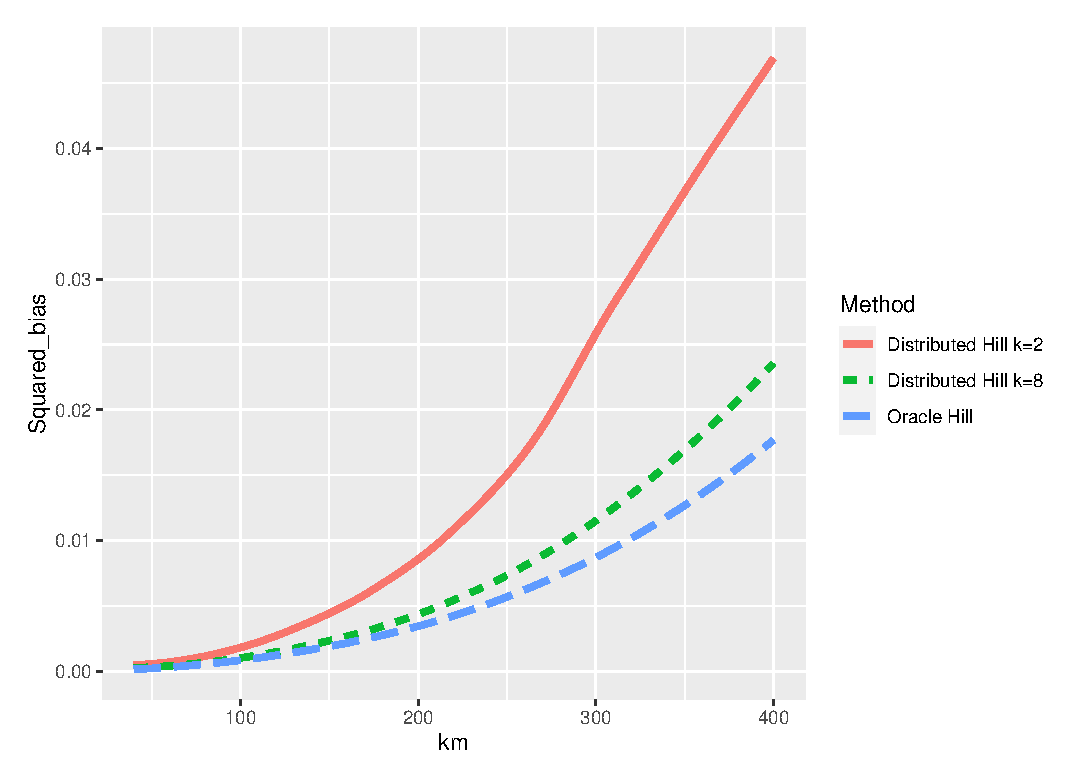
\includegraphics[width = 0.5\textwidth]{Simulation/Frechet_oracle_bias.eps} 
    \end{center}
    \begin{itemize}
        \item Unit Fr\'echet distribution ($\rho=-1$), $N=1000$
        \item We fix $k$ at two levels: $k=2$ and $k=8$.
        \item The x-axis is the effective number of exceedance ratios $km$.
    \end{itemize}

\end{frame}



\begin{frame}
    \frametitle{Simulation: variance for different level of $m$}
    \begin{center}
        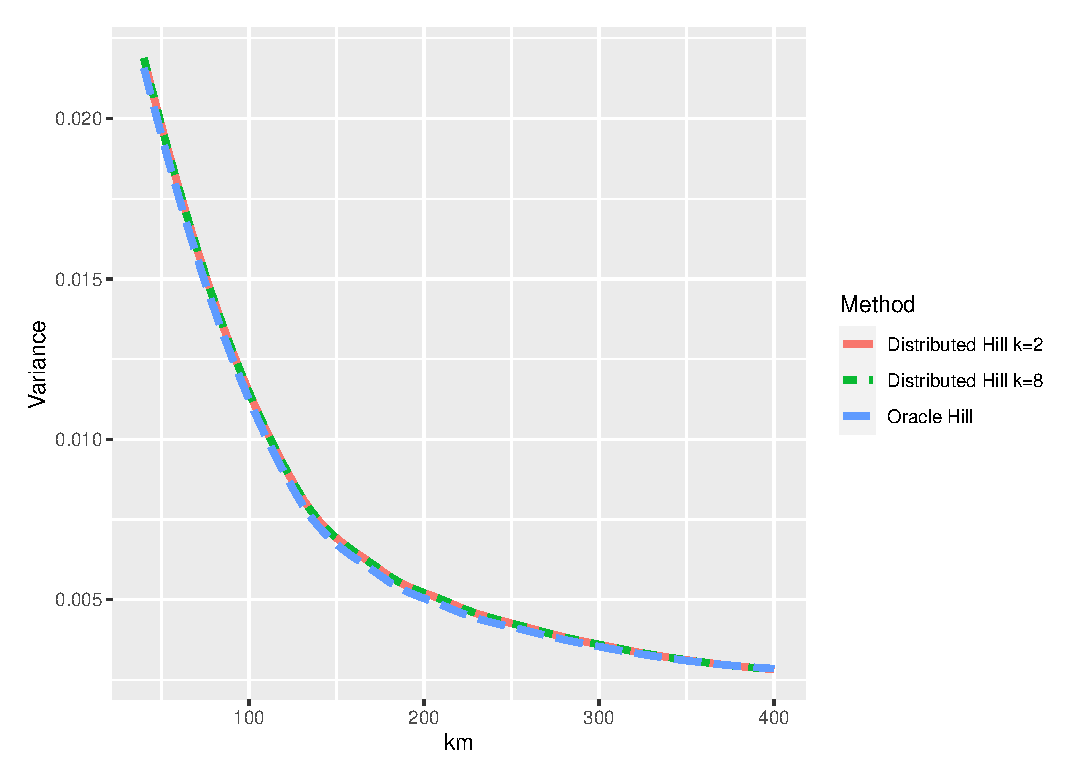
\includegraphics[width = 0.5\textwidth]{Simulation/Frechet_oracle_variance.eps}  
    \end{center}
    \begin{itemize}
        \item Unit Fr\'echet distribution ($\rho=-1$), $N=1000$
        \item We fix $k$ at two levels: $k=2$ and $k=8$.
        \item The x-axis is the effective number of exceedance ratios $km$.
    \end{itemize}

\end{frame}

\begin{frame}
    \frametitle{Simulation: MSE for different level of $m$}
    \begin{center}
         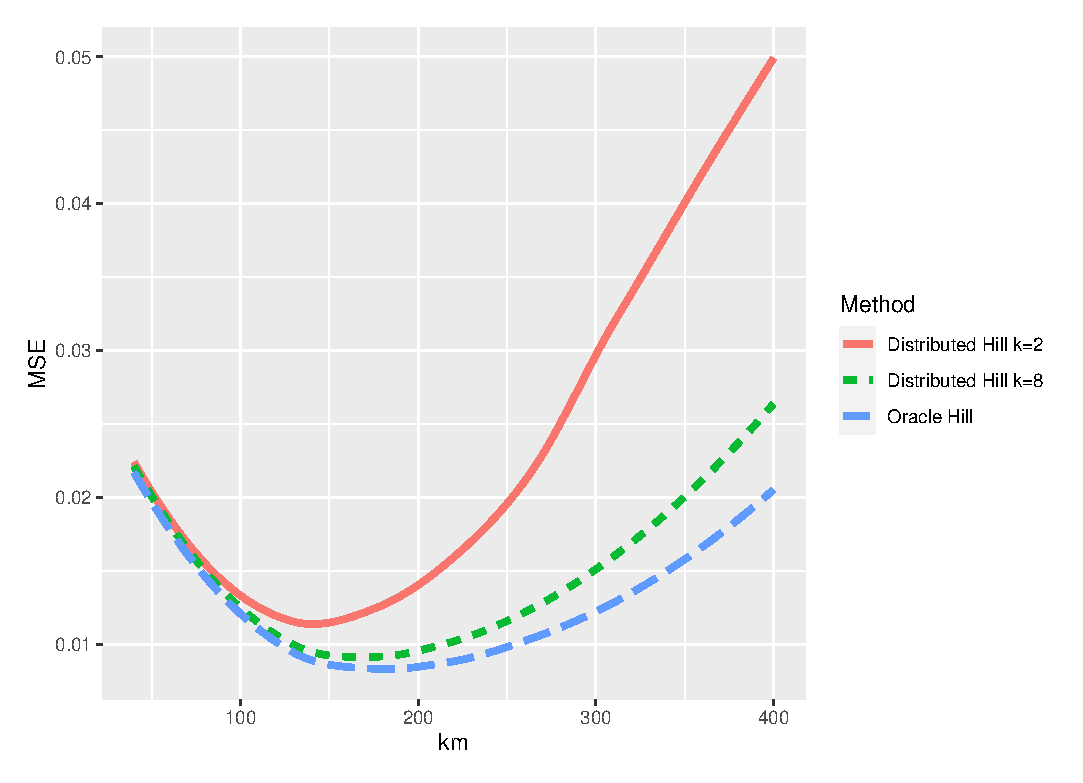
\includegraphics[width = 0.5\textwidth]{Simulation/Frechet_oracle_mse.eps} 
    \end{center}
    \begin{itemize}
        \item Unit Fr\'echet distribution ($\rho=-1$), $N=1000$
        \item We fix $k$ at two levels: $k=2$ and $k=8$.
        \item The x-axis is the effective number of exceedance ratios $km$.
    \end{itemize}

\end{frame}


\begin{frame}
    \frametitle{The choice of $k$}
\begin{itemize}

    \item The distributed Hill estimator is sensitive to the   choice of $k$ in each machine.
    \medskip
    \item This choice leads to a bias-variance tradeoff.
    \medskip
    \item Such a problem is more pronounced in the context of distributed inference.
\end{itemize}
    

\end{frame}

\begin{frame}
    \frametitle{The choice of $k$}
In extreme value statistics literatures, there are two types of solutions:
\bigskip
\begin{itemize}
    \item Finding the optimal level that balances the asymptotic bias and variance.
    
    \bigskip
    \item {\color{red} Bias correction.}
\end{itemize}
    

\end{frame}

\begin{frame}
    \frametitle{Bias Correction Methodology}

Recall that, for the distributed Hill estimator,
$$
\hat{\gamma}_{DH,k} -\gamma = \frac{N_{\gamma}}{\sqrt{km}}\frac{A(n/k)}{1-\rho}g(k,n,\rho)+\frac{1}{\sqrt{km}}o_P(1)
$$
    

\begin{itemize}
    \item The bias is an explicit function $\frac{A(n/k)}{1-\rho}g(k,n,\rho)$
    \medskip
    \item We shall estimate the bias, subtract it from the original estimator, and create the asymptotically unbiased distributed estimator.
\end{itemize}
\end{frame}


\begin{frame}
    \frametitle{Estimation for $\rho$}
\begin{itemize}
    \item We use a high intermediate sequence $k_{\rho}$ for estimating the second order parameter $\rho$.
    \medskip 
    \item Assume that as $N\to\infty$, $k_{\rho} \to\infty, k_{\rho}/n \to 0$, and 
    $$
  \begin{aligned}
    \sqrt{k_{\rho}m} A(n/k_{\rho})&\to\infty,\\
    \sqrt{k_{\rho}m} A^2(n/k_{\rho})&\to\lambda_1,\\
     \sqrt{k_{\rho}m} A(n/k_{\rho})B(n/k_{\rho})&\to\lambda_2,
  \end{aligned}
    $$
    where $B$ is the third order scale function.
\end{itemize}

\end{frame}

\begin{frame}
    \frametitle{Estimation for $\rho$}
Consider the following statistics computed based on the observations in each machine $j$,
$$
R_{j,k}^{(\alpha)} = \frac{1}{k}\sum_{i=1}^{k} \set{\log M_{j}^{(i)} -\log M_j^{(k+1)}}^{\alpha}, \quad \alpha=1,2,3.
$$

\begin{itemize}
    \item We request that each machine sends the values $R_{j,k}^{(\alpha)}, \alpha = 1,2,3$ to the central machine. 
    
    \item On the central machine, we take the average of the $R_{j,k}^{(\alpha)}$ to obtain 
    $$
    R_{k}^{(\alpha)} =\frac{1}{m}\sum_{j=1}^m R_{j,k}^{(\alpha)}
    $$
\end{itemize}

\end{frame}


\begin{frame}
    \frametitle{Estimation for $\rho$}
We define the estimator for the second order parameter $\rho$ as 
$$
\hat{\rho}_{k,\tau} = -3\abs{\frac{T_{k,\tau}-1}{T_{k,\tau}-3}},
$$
where 
$$
T_{k,\tau} := \frac{\suit{R_k^{(1)}}^{\tau}-\suit{R_k^{(2)}/2}^{\tau/2}}{\suit{R_k^{(2)}/2}^{\tau/2}-\suit{R_k^{(3)}/6}^{\tau/3}}.
$$
    

\end{frame}

\begin{frame}
    \frametitle{Asymptotically unbiased distributed estimator for $\gamma$}
    \begin{itemize}
        \item     We can choose a high level of $k$ in the eventual asymptotically unbiased distributed estimator.
        \item In our context, we choose $k_n$ such that,
        $$
            \begin{aligned}
                k_n/k_{\rho} & \to 0,\\
                \sqrt{k_{n}m} A(n/k_{n})&\to\infty,\\
                \sqrt{k_{n}m} A^2(n/k_{n})&\to 0,\\
                 \sqrt{k_{n}m} A(n/k_{n})B(n/k_{n})&\to 0.   
            \end{aligned}
        $$
    \end{itemize}

    

\end{frame}


\begin{frame}
    \frametitle{Asymptotically unbiased distributed estimator for $\gamma$}
The asymptotically unbiased distributed estimator for $\gamma$ is defined as 
$$
\tilde{\gamma}_{k_n,k_{\rho},\tau}:=R_{k_n}^{(1)} - \frac{R_{k_n}^{(2)}-2\suit{R_{k_n}^{(1)} }^2 }{2R_{k_n}^{(1)} \hat{\rho}_{k_{\rho},\tau}\suit{1-\hat{\rho}_{k_{\rho},\tau}}^{-1}}.
$$
    

Note that, the estimator $\tilde{\gamma}_{k_n,k_{\rho},\tau}$ adheres to a DC algorithm since each machine only sends five values $\set{R_{j,k_n}^{(1)},R_{j,k_n}^{(2)},R_{j,k_n}^{(3)},R_{j,k_{\rho}}^{(1)},R_{j,k_{\rho}}^{(2)}}$ to the central machine.

\end{frame}
\begin{frame}
    \frametitle{Asymptotics}
{\bf Theorem} 

Under some mild conditions, 
$$
\sqrt{k_nm}\suit{\tilde{\gamma}_{k_n,k_{\rho},\tau}-\gamma}
\stackrel{d}{\to} N\suit{0,\gamma^2\set{1+(\rho^{-1}-1)}^2}.
$$
    

\end{frame}


\begin{frame}
    \frametitle{Simulation: Absolute bias for different levels of $k_n$}
\begin{center}
     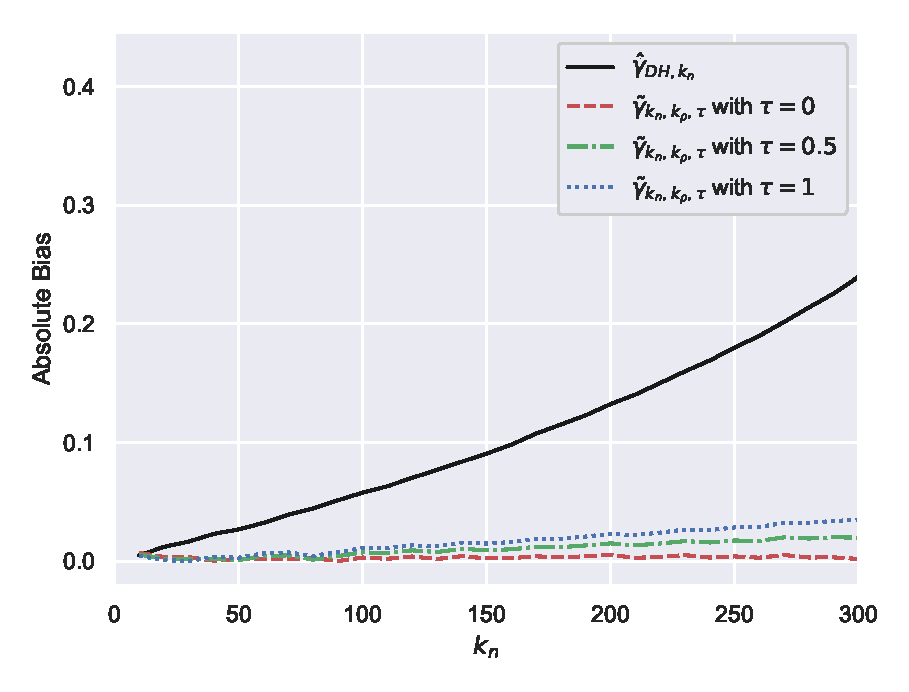
\includegraphics[width=0.65\textwidth]{program/simu1/figs/Frechet_m20_0.eps}
\end{center}
    \vspace{-2ex}
    \begin{itemize}
        \item Unit Fr\'echet distribution ($\rho = -1$)
        \item  $N = 10000, m=20$
    \end{itemize}

\end{frame}


\begin{frame}
    \frametitle{Simulation: Absolute bias for different levels of $k_n$}
\begin{center}
    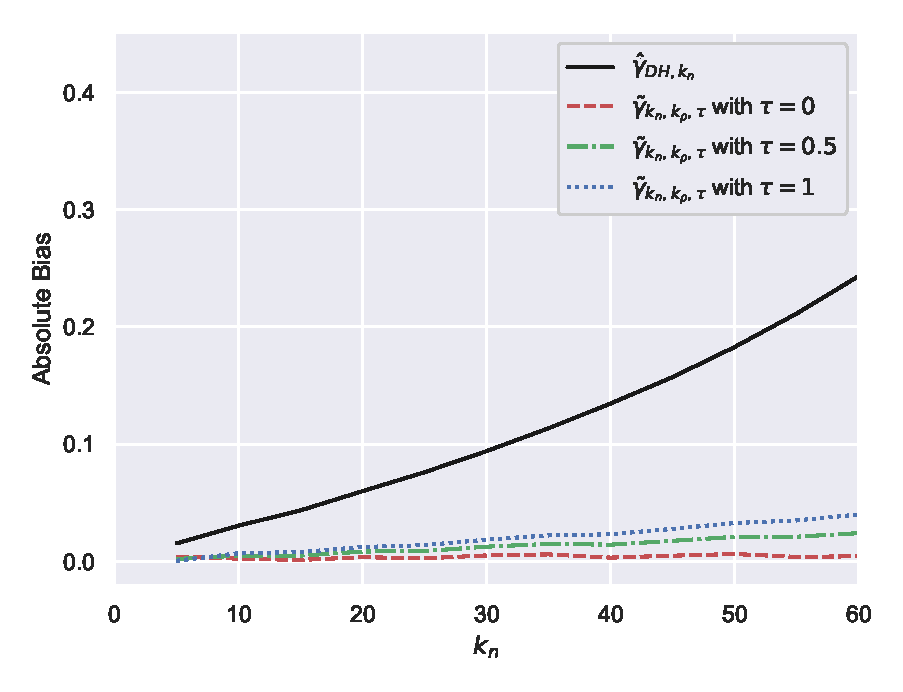
\includegraphics[width=0.65\textwidth]{program/simu1/figs/Frechet_m100_0.eps}
\end{center}
\vspace{-2ex}
\begin{itemize}
    \item Unit Fr\'echet distribution ($\rho = -1$)
    \item  $N = 10000, m=100$
\end{itemize}
\end{frame}


\begin{frame}
    \frametitle{Simulation: Absolute bias for different levels of $k_n$}
\begin{center}
    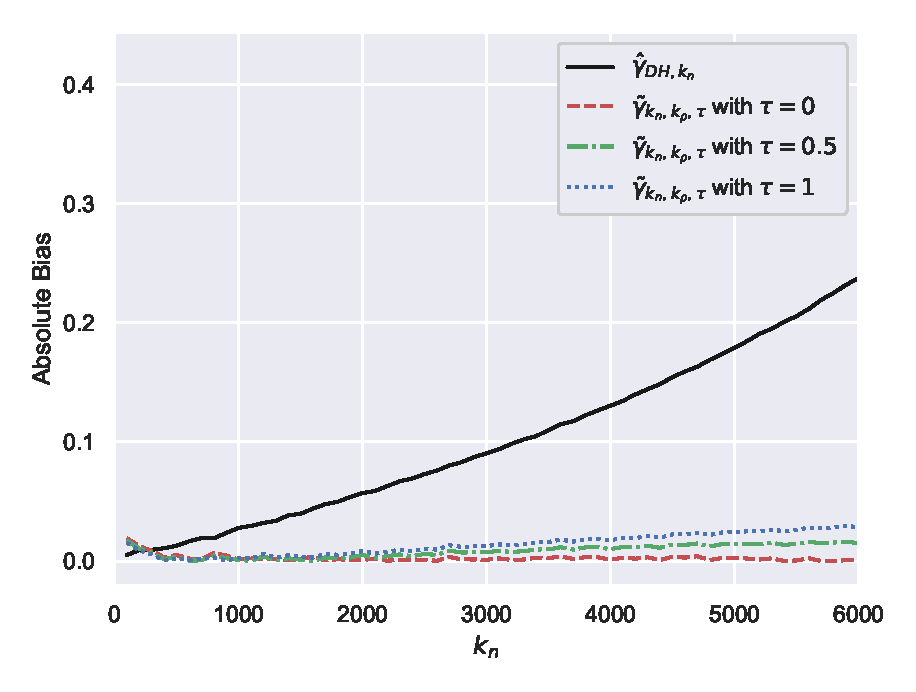
\includegraphics[width=0.65\textwidth]{program/simu1/figs/Frechet_m1_0.eps}
\end{center}
\vspace{-2ex}
\begin{itemize}
    \item Unit Fr\'echet distribution ($\rho = -1$)
    \item  $N = 10000, m=1$
\end{itemize}
\end{frame}

\begin{frame}
    \frametitle{}

    \begin{center}
        {\LARGE  Thank You!}
    \end{center}

\end{frame}
\end{document}